\chapter{Graphical User Interface} \label{chap:GUI}

The web was chosen as the visualization environment for its simplicity and the number of possible tools to use. The website is available at the public IP address http://147.228.124.230:8881/. The pages are written in separate HTML files and share the same JavaScript and CSS file. JavaScript is used to provide the necessary dynamics, such as new sensor's data, which display on the page or changes the sensor's state icon. The web design is defined in the CSS file. Styles for HTML elements are stored here, such as font letters, font family, the layout of elements on the page. Combining these three languages was created an interactive web visualization for the presentation of measured data and control of a smart home. Libraries and frameworks used to build the website are Bootstrap, JQuery and Dygraphs (described in \cref{section:libraries_and_frameworks}).

The structure of the website is divided into subpages such as Home, Analytics, Modules. The user can move between these subpages using the horizontal menu (see \cref{fig:screenshot_menu}), which consists of three buttons with subpage names. The style of this navigation menu is designed using the Bootstrap framework. This menu is changed to a slider from above for more straightforward operation using the touch screen when using a mobile device.

\begin{figure}[H]
    \centering
    
\includegraphics[width=\textwidth]{img/screenshot_menu.png}
    \caption{Screenshot of the horizontal menu on the web page}
    \label{fig:screenshot_menu}
\end{figure}

When a user opens a web page, all modules, voice commands and currently connected controller are loaded using the REST service. This information is transmitted in JSON format. The connected controller always shows in the navigation menu next to links of subpages.

The Home page allows the user to interact with the light control, view the current status of the sensors, current data from the sensors, the voice commands currently in use, and display the fundamental weather forecast for today and tomorrow. The Analytics page offers the user detailed historical data from sensors after selecting sensors using the switch at the sensors filter section and sending a query using the submit button. The data from the database display on the page below the sensors filter. The Modules page shows the user all the programmed modules user can use with all its voice commands. It is possible to switch each of these modules on/off using the switch next to the module name.

\section{Libraries and frameworks} \label{section:libraries_and_frameworks}

which facilitate work and make the page more robust. These libraries and frameworks are widely used and known to all in web development. 


\section{Home}

The Home page is the default page when the website is visited. At the top of the page is a menu with links to other pages. Below the menu is the main container with all the information on the page. This container is divided into smaller boxes, which will be described below.

% \begin{figure}[H]
%     \centering
%     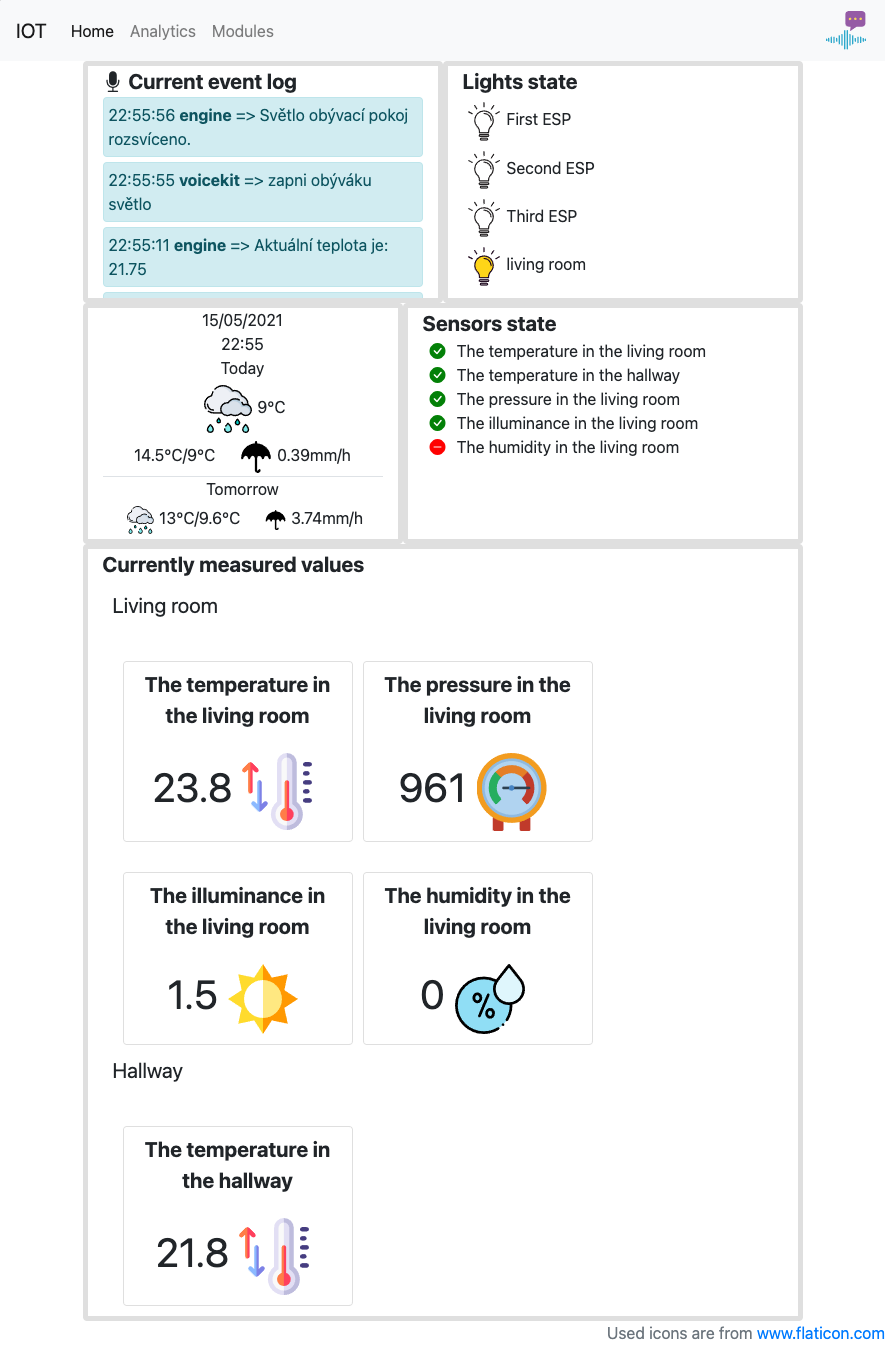
\includegraphics[width=\textwidth]{img/web_home.png}
%     \caption{Screenshot of the web page on the Home page}
%     \label{fig:web_home}
% \end{figure}

The first box here is the Current event log (see \cref{fig:screenshot_home_current_event_log}), the currently spoken voice commands are displayed here. It shows the time of the message and from whom the message is. 

\begin{figure}[H]
    \centering
    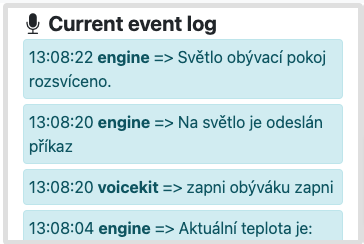
\includegraphics[width=0.7\textwidth]{img/screenshot_home_current_event_log.png}
    \caption{Screenshot of the Current event log box on the Home page}
    \label{fig:screenshot_home_current_event_log}
\end{figure}

The box next to the Current event log box is Lights state box (see \cref{fig:screenshot_home_lights_state}). All connected lights with an image of a bulb are listed in this box. The bulb indicates whether the light is turned on, off or not connected. When the bulb image is pressed, the light turns on or off, depending on the initial state.

\begin{figure}[H]
    \centering
    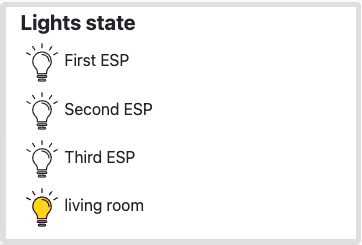
\includegraphics[width=0.7\textwidth]{img/screenshot_home_lights_state.png}
    \caption{Screenshot of the Lights state box on the Home page}
    \label{fig:screenshot_home_lights_state}
\end{figure}

The box below the Current event log is Weather (see \cref{fig:screenshot_home_weather}). This box shows the fundamental weather forecast for today and tomorrow. At the top is placed current date and time. Below time is displayed forecast for today, which contains icons that specify weather type (such as rain, sun, fog, snowfall). Next to the icon is today's forecast temperature. The row below shows a forecast temperature for a day temperature and night temperature with a rain volume displayed next to that. The last row in this box display day temperature, night temperature and rain volume for tomorrow.

\begin{figure}[H]
    \centering
    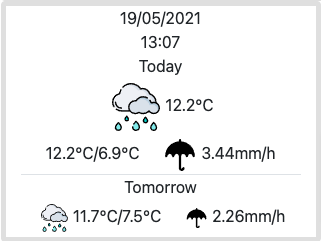
\includegraphics[width=0.7\textwidth]{img/screenshot_home_weather.png}
    \caption{Screenshot of the Weather box on the Home page}
    \label{fig:screenshot_home_weather}
\end{figure}

The box on the left of the Weather box is the Sensors state box (see \cref{fig:screenshot_home_sensors_state}). This box show sensor's indicator and description. The indicator is red when the sensor working not correctly and is an error in data, or the sensor did not respond for 5 minutes. Otherwise, the indicator is green.

\begin{figure}[H]
    \centering
    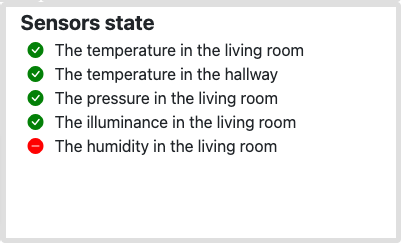
\includegraphics[width=0.8\textwidth]{img/screenshot_home_sensors_state.png}
    \caption{Screenshot of the Sensors state box on the Home page}
    \label{fig:screenshot_home_sensors_state}
\end{figure}

The last box on the page is the Currently measured values box (see \cref{fig:screenshot_home_currently_measured_values}). This box shows current data from sensors that arrange by rooms.

\begin{figure}[H]
    \centering
    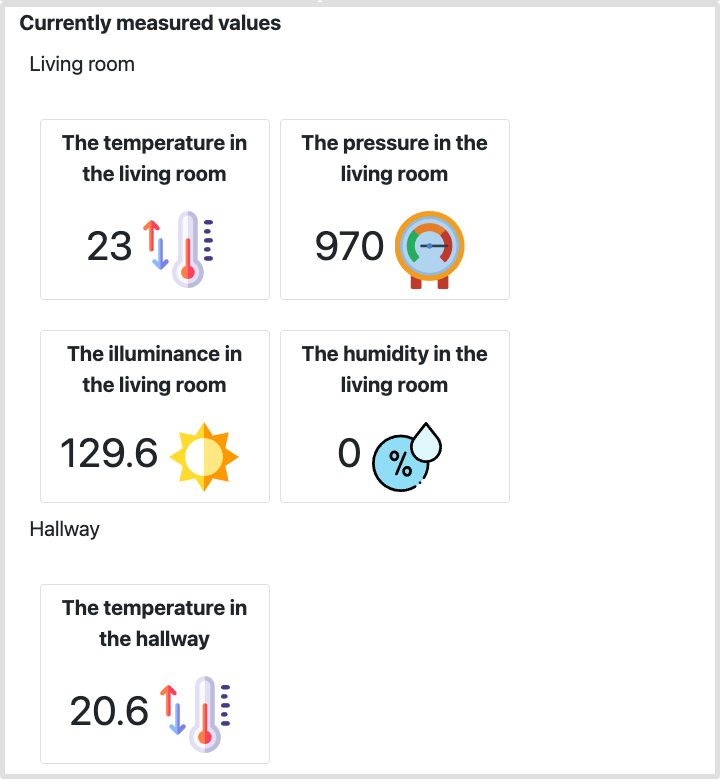
\includegraphics[width=\textwidth]{img/screenshot_home_currently_measured_values.png}
    \caption{Screenshot of the Currently measured values on the Home page}
    \label{fig:screenshot_home_currently_measured_values}
\end{figure}

All values from ESP on this page are changed asynchronously according to the new data arriving at the server.

\section{Analytics}

The Analytics page allows user to select specific sensors and visualize their historical values stored in the MongoDB database. When the user opens the page, all data from the engine are immediately sent to the page using WebSocket. The user's first step in entering the page is to select the sensors in the list of sensors (see \cref{fig:screenshot_analytics_filter}) he wants to plot below (see \cref{fig:screenshot_analytics_graph}). After filling in these preferences, the user clicks the submit button "Vykreslit data". At this point, the page begins to transform the received data into the desired Dygraph library format. The Dygraph library was chosen based on the benefits of an open-source license and easy selection of the time user want to display data. The time is selected using the banner below the graph by dragging the wick.

\begin{figure}[H]
    \centering
    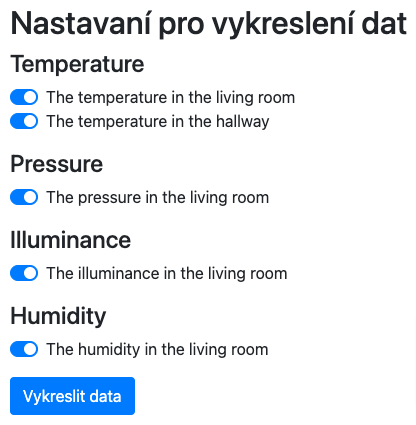
\includegraphics[width=0.7\textwidth]{img/screenshot_analytics_filter.png}
    \caption{Screenshot of the Sensors selection list on the Analytics page}
    \label{fig:screenshot_analytics_filter}
\end{figure}

\begin{figure}[H]
    \centering
    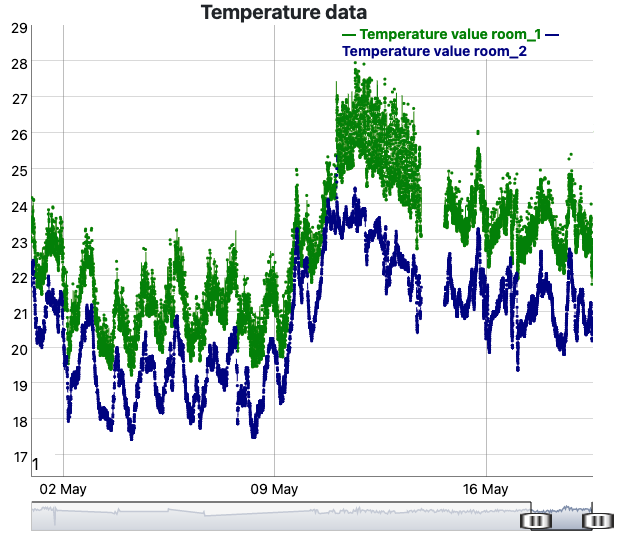
\includegraphics[width=\textwidth]{img/screenshot_analytics_graph.png}
    \caption{Screenshot of the temperature graph on the Analytics page}
    \label{fig:screenshot_analytics_graph}
\end{figure}

\section{Modules} \label{section:modules}

The Modules page allows the user to view all possible voice commands for each module. On the left is a list of all modules (see \cref{fig:screenshot_modules_modules}) that connect to the engine. After clicking on the user-selected module, the module name, module description and list of blocks of all possible voice commands display on the left side of the page (see \cref{fig:screenshot_modules_calls}). The function's name to execute, the description of the command and all possible calls display in the block of voice command.

The following functionality is turning on or off the module. The module turns by clicking the switch next to the module's name in the list of modules. The click sends the message to the engine by WebSocket then the module is moved from the list of modules to the list of modules turned off.

\begin{figure}[H]
    \centering
    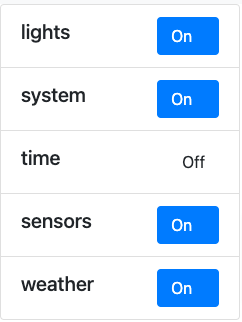
\includegraphics[width=0.4\textwidth]{img/screenshot_modules_modules.png}
    \caption{Screenshot of the list of all modules on the Modules page}
    \label{fig:screenshot_modules_modules}
\end{figure}

\begin{figure}[H]
    \centering
    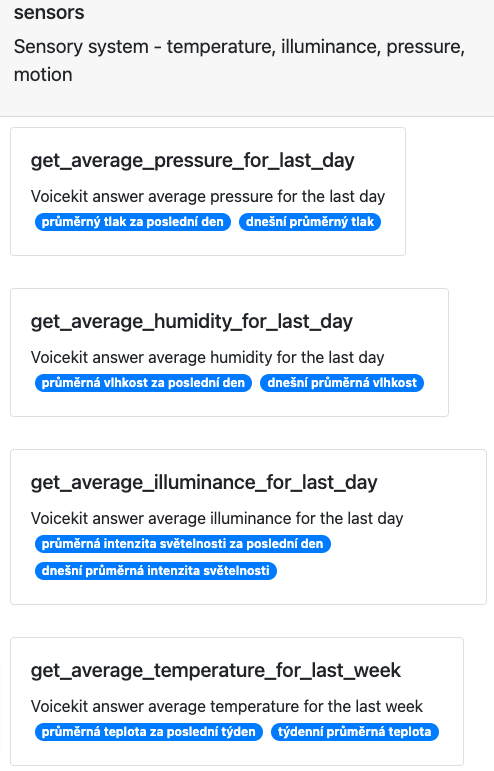
\includegraphics[width=0.9\textwidth]{img/screenshot_modules_calls.png}
    \caption{Screenshot of the list of calls for the module Sensors on the Modules page}
    \label{fig:screenshot_modules_calls}
\end{figure}


